%ProblemSheet1.tex

% DOCUMENT CLASS:
% Two sided, icelandic
\documentclass[english,a4paper,twoside]{amsart}
%\documentclass[icelandic,a4paper,twoside,draft]{amsart}
%\documentclass[icelandic,a4paper,twoside]{article}
%\documentclass[icelandic,a4paper,twoside,draft]{article}
\usepackage[pdftex]{color,graphicx} %Used for inputting pdf graphics into document

% Enable for hyperlinks in the file THIS MUST BE THE LAST COMMAND IN THE PREAMBLE TO WORK!
\usepackage[pdftex]{hyperref}
\usepackage{tikz}
\usepackage[english]{babel}
%\usepackage[icelandic]{babel}
\usepackage[T1]{fontenc}
\usepackage[utf8]{inputenc}

% Fancy enumerate environment
\usepackage{enumerate}
\usepackage{multicol}

% For defining your own environments
\usepackage{amsthm}

\theoremstyle{lemma}
\newtheorem{problem}{Problem}
\newtheorem*{solution}{Solution}
\newtheorem{conj}{Conjecture}
\newtheorem{lemma}{Lemma}

\usepackage{mathtools}
\DeclarePairedDelimiter{\ceil}{\lceil}{\rceil}
\DeclarePairedDelimiter{\floor}{\lfloor}{\rfloor}

\usepackage{fullpage}
\usepackage{pdfpages}

% My macros
\newcommand{\myd}{\mathrm{d}}
\newcommand{\NN}{\mathbb{N}}
\newcommand{\ZZ}{\mathbb{Z}}
\newcommand{\inv}{\mathrm{inv}}
%--------------------------------------------------------------------------------

% Starting document
\begin{document}

\title[exesefsfe]{Extensions of Grundy's Game}

\author{Pétur Orri Ragnarsson}

\date{\today}

\maketitle

\thispagestyle{empty}

\section{Grundy's Game}
Grundy's Game is well known in game theory. Two players begin with a pile of coins.
The first player splits the pile into two uneven piles. The second player picks one of the
piles and splits it into two uneven piles. The first player then picks one of the three piles
and splits it into uneven piles. This goes on until no more uneven splits can be made. The
last player to move wins.

Grundy's Game has been studied extensively and although some patterns have been found
in its SG-values\footnote{See for example \emph{Winning Ways for Your Mathematical Plays}, page 111.},
no one has been able to come up with an overall description of them
that does not involve examining the whole game tree.

\section{Extending Grundy's Game}
We present two ways extend Grundy's game by allowing more splits and solve some cases.

\section{Fixed number of splits}
We can extend the game such that for a given natural number $M \geq 2$ at each turn the
pile must be split into \emph{exactly} $M$ piles, no two of which have the same size.

\subsection{Upper bound}
It is obvious that if we have a pile of size $n < \sum_{i=0}^{M} i = \frac{M(M+1)}{2}$ that it is
not possible to split it into $M$ uneven piles. Therefore, for such $n$, $g(n) = 0$.
However with $n = \frac{M(M+1)}{2}$, the split $1, 2, ..., M$ is valid and will have SG-value 1,
since the SG-values of all the smaller piles are 0.

\begin{lemma}
    The first non-zero SG-value appears at pile size $n = \frac{M(M+1)}{2}$.
\end{lemma}

We now want to prove that the SG-values cannot increase faster than once for every
$\sum_{i=1}^{M-1} i = \frac{(M-1)M}{2}$ increases in $n$, the pile size. We know that the first value
of 1 appears at pile size $\frac{M(M+1)}{2}$. To get the first value of 2 we must have a split where
at least one of the piles
has a value of 1. Therefore at least one pile must be of size at least $\frac{M(M-1)}{2}$. The minimum sizes of
the remaining piles that give a valid split are $1, 2, ..., M-1$, so the minimum pile size where SG-value 2
can appear is $\frac{M(M+1)}{2} + \frac{(M-1)M}{2}$, and it does, since all the small piles
have SG-value 0.

\begin{lemma}
    The first SG-value larger than 1 is 2 and appears at pile size $\frac{M(M+1)}{2} + \frac{(M-1)M}{2}$.
\end{lemma}

To get further we need the following conjecture that says we don't "skip" any SG-values:

\begin{conj}
\label{conj:noskip}
    If a pile of size $n$ has SG-value $k > 0$, then there is a pile of size $n' < n$ with
    SG-value $k-1$.
\end{conj}

Let us now assume that for all piles up to a given $n$, the SG-values increase at most at the rate
of one every $\frac{(M-1)M}{2}$ increases in pile size. Further assume that $n$ is the smallest pile
that has a given SG-value $k$. Then we want to show that the smallest possible pile size $m$ that has
SG-value $k+1$ is $m = n+\frac{(M-1)M}{2}$.

\subsection{Upper bound can be reached for \emph{M} > 3}
Now we want to show that we can reach the upper bound for $M > 3$. Let $n$ be some pile and $k$ be
it's upper bound according to the previous section. Let $0 \leq l < k$. We will show that we can
split $n$ such that the new piles together have SG-value $l$.

First find the smallest pile $n'$ with SG-value $l$. That is our first pile. We will then split the
remaining coins into $M-1$ piles such that their total values are 0. If $M-1$ is odd, then take
one coin and put it in its own pile. It has SG-value 0. We now have an even number $m$ of piles remaining
to fill. Split the remaining coins as evenly as possible into these piles. That means that the
pile sizes are a sequence $n_1, n_2, ..., n_m$ such that $n_i - n_{i-1} = 1$ for all $i$ except
possibly one, where the difference is 2.

These $m$ piles can have at most 2 different SG-values according to the induction hypothesis,
since $M < \frac{(M-1)M}{2}$ for all $M > 3$ ($M$ is the largest possible difference between the sizes).
If all the piles have the same size, then their SG-values cancel out and we are done.
Further, if they have two different SG-values but there's an even number of piles for each value, they
also cancel out and we are done.

If we are not done yet, then there is an odd number of piles with each SG-value.
We will fix this by modifying the two largest piles with the lower SG-value. We remove $\frac{(M-1)M}{2} - 3$
coins from the smaller of these two piles. That will change it from being the second biggest possible
pile with this SG-value to being the second smallest. The other, larger, pile will increase in SG-value.
See figure \ref{fig:explanation}.
Thus we now have an even number of piles with each SG-value. Note that this operation will not
change these piles into piles of a size already taken, since we move them far enough.
If there is only one pile with the smaller SG-value, we use the two smallest piles with the
higher SG-value instead.

There are two cases to consider where we still have piles of even size. The first one is when one of the
remainder piles is of size 1 and therefore collides with the special pile of size one. If this happens,
then the remainder piles must be of sizes $1, ..., M-2$, which means we're trying to create
an SG-value that is in fact not possible to create, ie $l \geq k$. That's nonsense so we don't need
to worry about that.

The other case is where the original pile is equal in size with one of the remainder piles. Then these
piles are the smallest piles with this SG-value. We cancel the whole process and start over, but this
time we pick the first pile to be the largest one with its SG-value. That guarantees that the remainder
piles cannot collide with it. The rest of the process is the same.

\subsection{\emph{M} = 3}
Clearly from the data, the previous does not hold for $M=3$ (see fig. \ref{fig:fixed3_long}).
The proof fails when the two remainder
piles are of an uneven size and do not have the same SG-value. We cannot as easily move coins around
in that case. For example, the first $n$ to fail is 13. With the previous method the split would be
$1 - 5 - 7$, with respective SG-values $0 - 0 - 1$ and no way to apply the method.

However, there is an apparent pattern by looking at the plot of the first
2000 values. Most of the values below the main line appear to be on a line of their own. I haven't
been able to figure out what the pattern is.

\section{Bounded number of splits}
We can also extend the game such that we allow the players to choose how many piles to split into,
with an upper limit $M$ on the number of piles.

\subsection{$\emph{M} > 4$}
\begin{conj}
\label{conj:any4plus}
The SG-value for a pile of size $n \geq 9$ is $n-4$.
For smaller piles the SG-values can be read from figure \ref{fig:any5}.
\end{conj}

Note that if we believe conjecture \ref{conj:noskip} (no skipping values) also applies in this
extension of the game, then it is enough to prove this for the case $M = 5$. The conjecture implies
that the SG-value increases at most by one for every increase in pile size. Since conjecture
\ref{conj:any4plus} says we do indeed reach that slope, the larger cases can simply choose the
splits from the $M=5$ case.

\subsection{\emph{M} = 4}
The SG-value for a pile of size $n\geq 17$ appears to be $n-5$.
The smaller values can be read from figure \ref{fig:any4}.
This case is different from the larger ones due to $n=17$ where a 5-way split is needed to achieve
the SG-value 0.


\section{Open questions}

When $M=3$ we can see from figs. \ref{fig:any3_long} and \ref{fig:fixed3_long} that most values
seem to follow a linear trend for both games. However, there
are a few values that don't follow this trend. Is there a pattern to these and is it similar to
the rare and common value pattern seen in the regular version of Grundy's game.

In the $M=3$ case, some SG-values are repeated. What is the pattern of these repetitions?

Both of the extensions simplify to Grundy's game when $M=2$. Can what we know of the higher
$M$s give us insight into Grundy's game?



\newpage

\begin{figure}
    \caption{Graphical explanation of a splitting process.}
    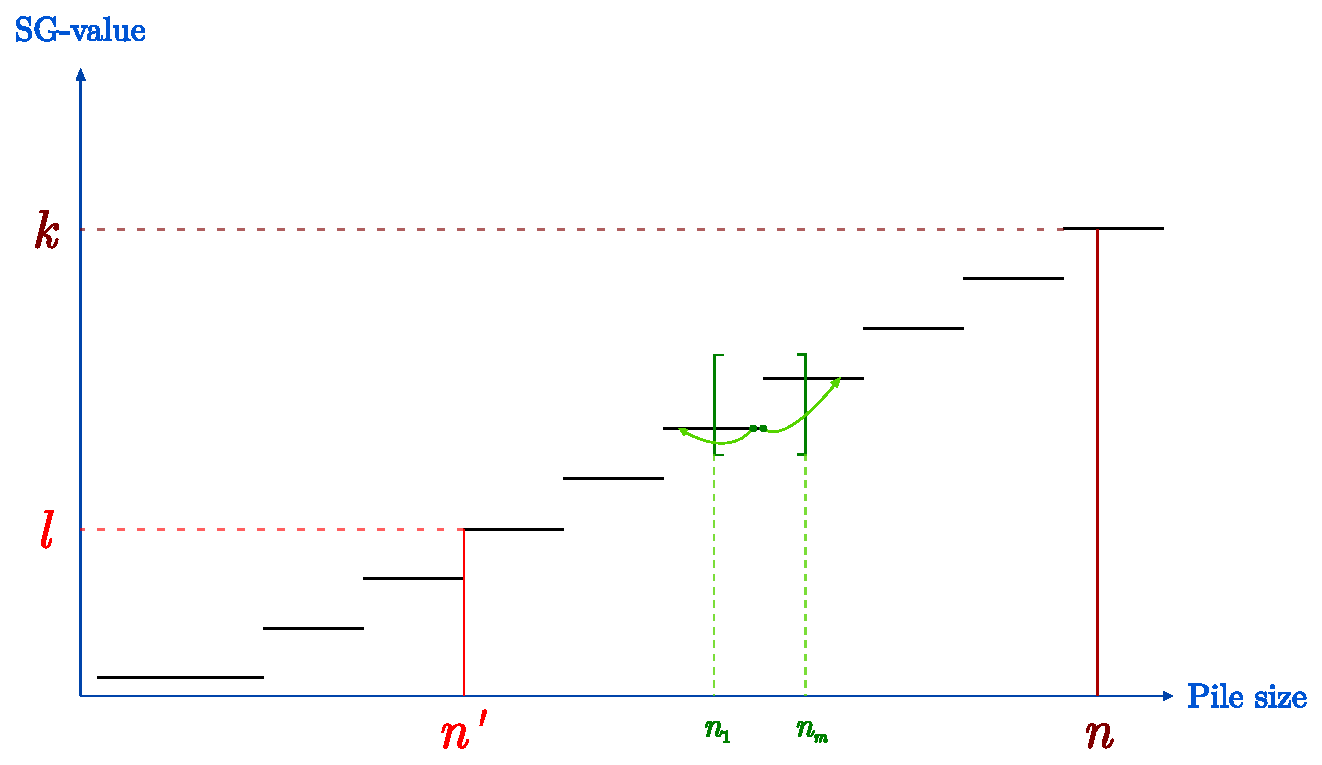
\includegraphics[width=\linewidth]{explanation.pdf}
    \label{fig:explanation}
\end{figure}

\begin{figure}
    \caption{SG-values where up to 4 splits are allowed.}
    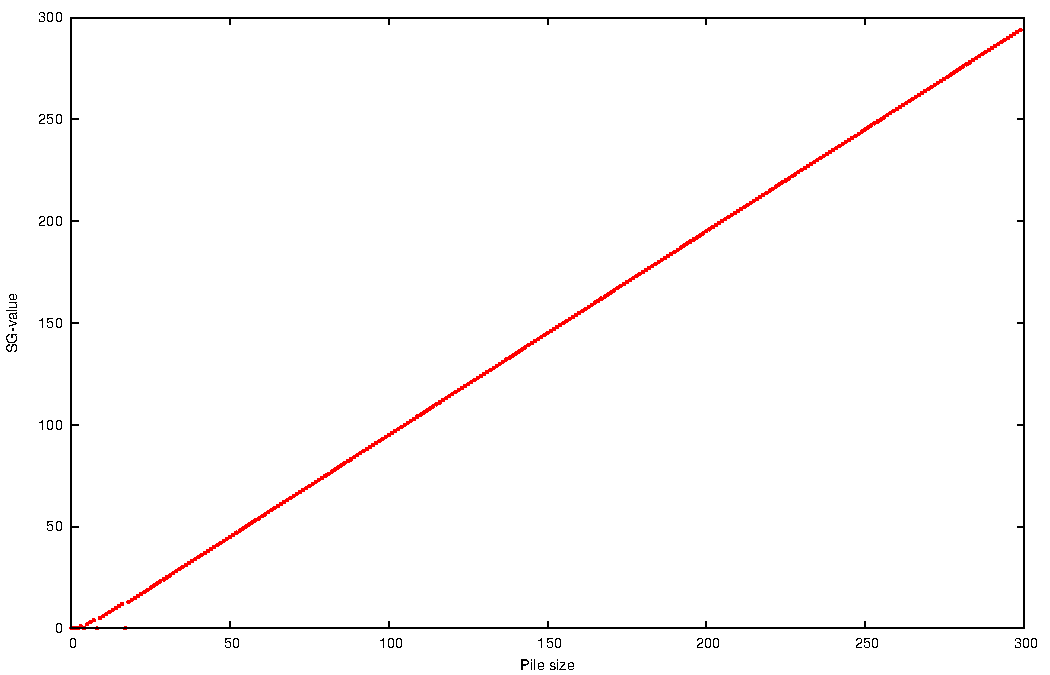
\includegraphics[width=\linewidth]{../plots/any4.pdf}
    \label{fig:any4}
\end{figure}

\begin{figure}
    \caption{SG-values where up to 3 splits are allowed.}
    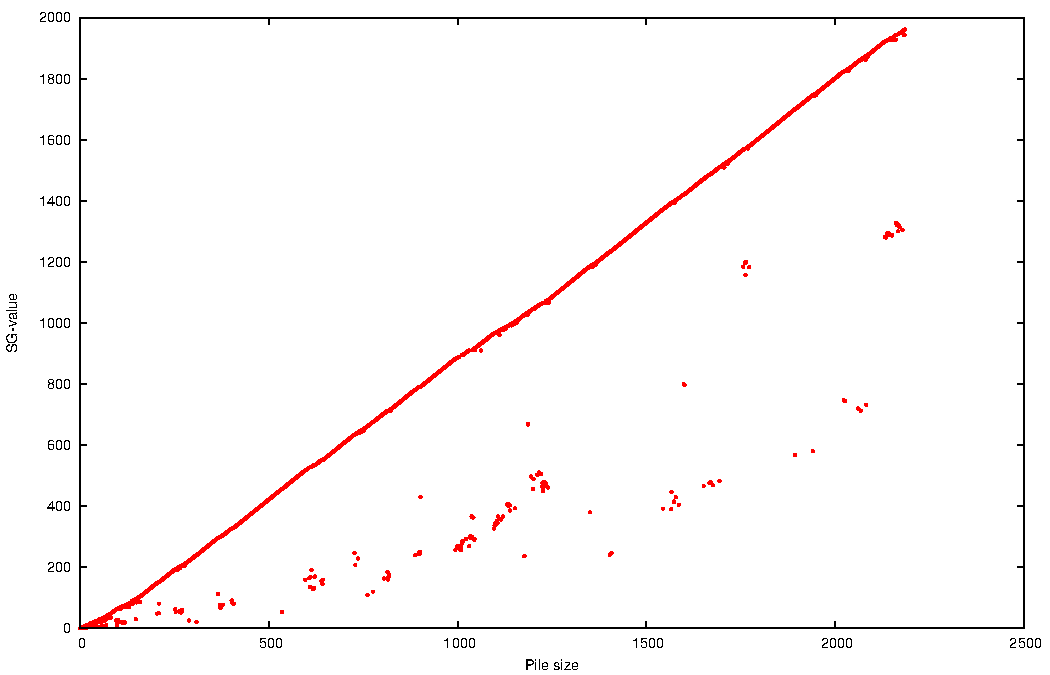
\includegraphics[width=\linewidth]{../plots/any3_long.pdf}
    \label{fig:any3_long}
\end{figure}

\begin{figure}
    \caption{SG-values where exactly 3 splits are allowed.}
    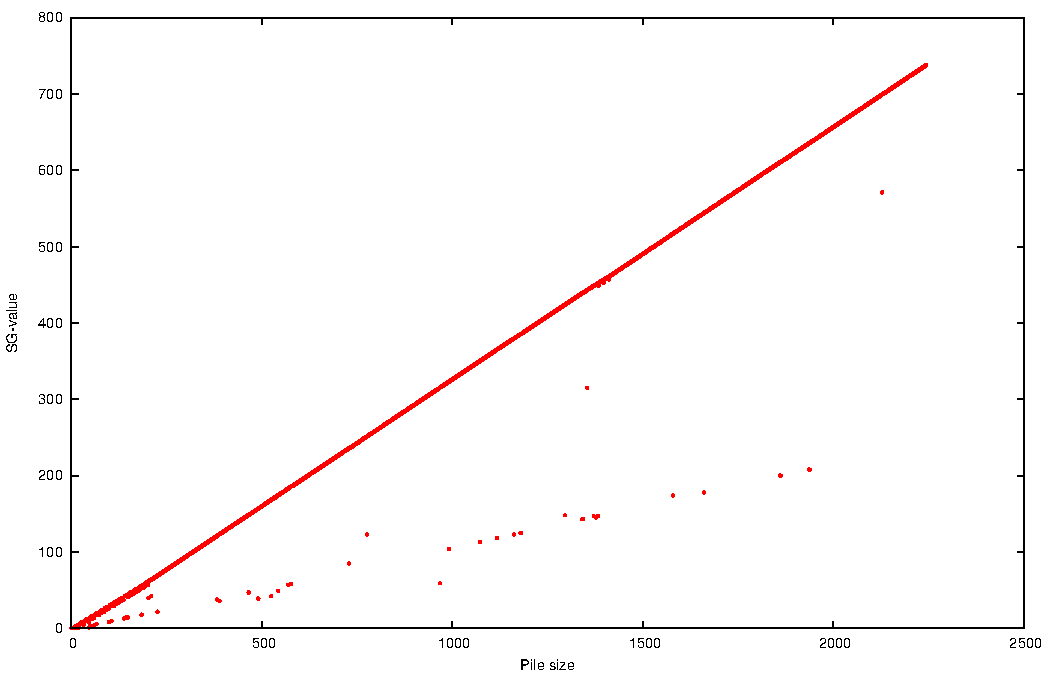
\includegraphics[width=\linewidth]{../plots/fixed3_long.pdf}
    \label{fig:fixed3_long}
\end{figure}

\begin{figure}
    \caption{SG-values where up to 5 splits are allowed.}
    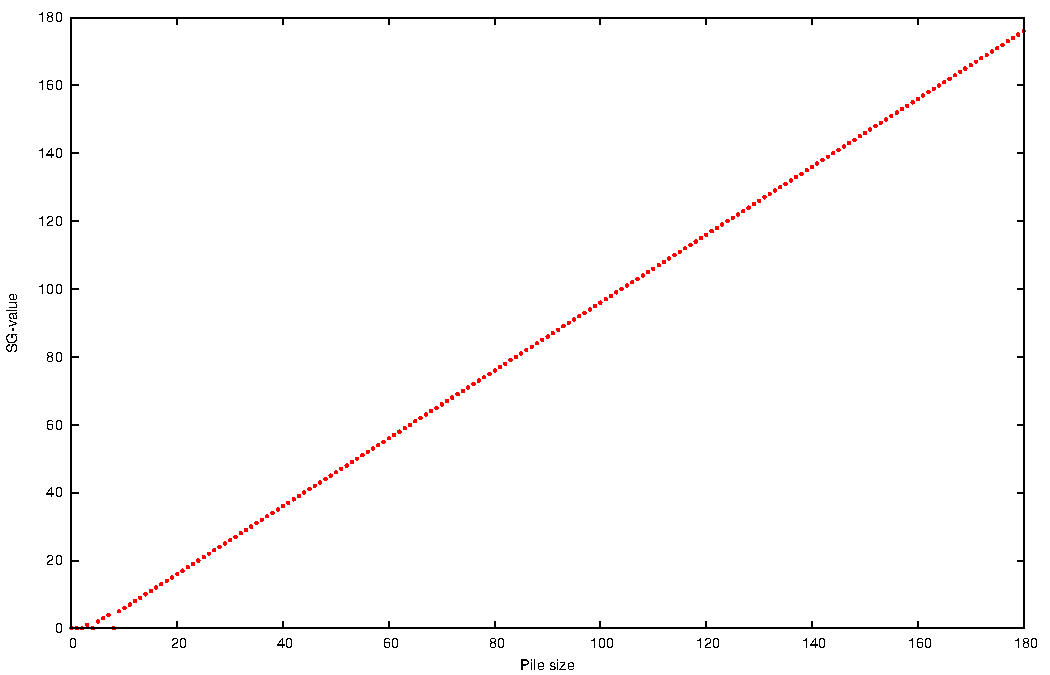
\includegraphics[width=\linewidth]{../plots/any6.pdf}
    \label{fig:any5}
\end{figure}

\begin{figure}
    \caption{SG-values exactly 5 splits are allowed.}
    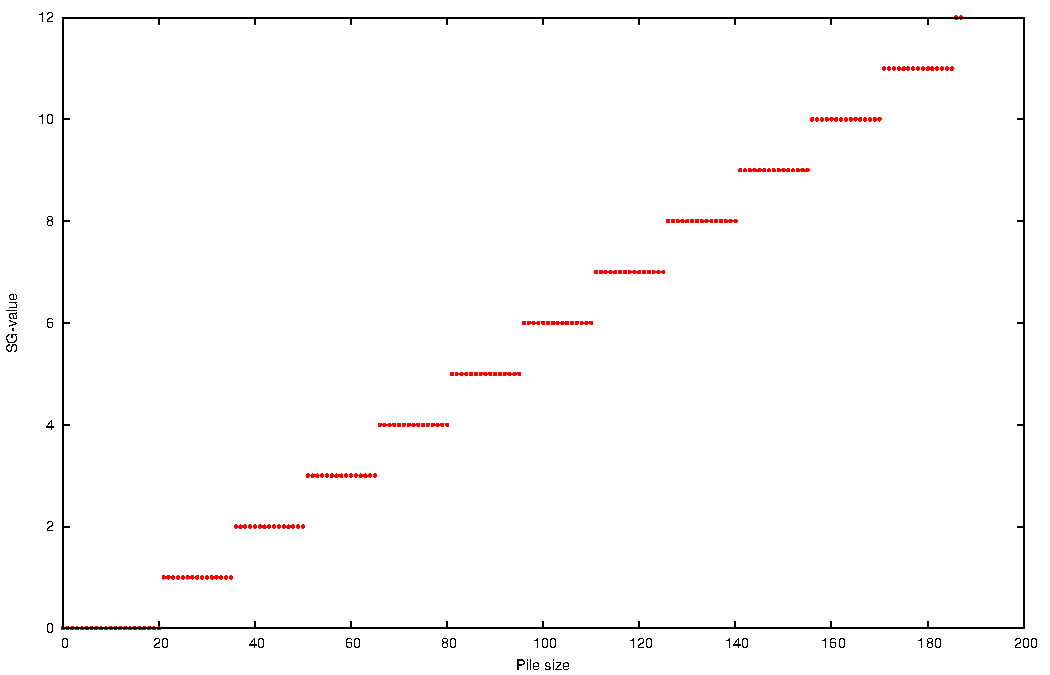
\includegraphics[width=\linewidth]{../plots/fixed6.pdf}
    \label{fig:fixed5}
\end{figure}

\end{document}























